\documentclass[11pt,letterpaper]{article}
\usepackage[lmargin=1in,rmargin=1in,tmargin=1in,bmargin=1in]{geometry}
\usepackage{../style/quiz}
\setbool{hideans}{false} % Student: True; Instructor: False

% -------------------
% Content
% -------------------
\begin{document}
\quiz{8}

% Problem 1
\problem If $f(x)= 5x + 8$ and $g(x)= x^2 - 4$, compute $(f \circ g)(-1)$. \pspace

\ans{We know that $(f \circ g)(-1)= f \big( g(-1) \big)$. But\dots
	\[
	\begin{aligned}
	g(-1)&= (-1)^2 - 4= 1 - 4= -3 \\
	f(-3)&= 5(-3) + 8= -15 + 8= -7
	\end{aligned}
	\]
Therefore, we have\dots
	\[
	(f \circ g)(-1)= f \big( g(-1) \big)= f(-3)= -7
	\]
}



% Problem 2
\problem Consider the function $h(x)= 4(x + 5)^3$. Find functions $f(x)$ and $g(x)$ such that $h(x)= f \big( g(x) \big)$, i.e. write $h(x)$ as a composition of two functions. \pspace

\ans{There are infinitely many answers. For instance, we have\dots
	\[
	\begin{aligned}
	f(x)&= 4x^3 \\
	g(x)&= x + 5
	\end{aligned}
	\]
We can verify that this selection works:
	\[
	f \big( g(x) \big)= f(x + 5)= 4(x + 5)^3= h(x)
	\]
}



% Problem 3
\problem Compared to the graph of $f(x)$, what does the graph of $4 - f(x + 6)$ `look like'? \pspace

\ans{We know that the graph of $f(x + 6)$ is the graph of $f(x)$ shifted 6~units to the left. The graph of $-f(x + 6)$ is the graph of $f(x + 6)$ reflected through the $x$-axis. Finally, the graph of $4 - f(x + 6)= -f(x + 6) + 4$ is the graph of $-f(x + 6)$ shifted 4~units upwards. Therefore, the graph of $4 - f(x + 6)$ is the graph of $f(x)$ shifted 6~units to the left, reflected through the $x$-axis, and then shifted 4~units upward.} \vfill



% Problem 4
\problem Does the function $f(x)$ given below have an inverse? Explain. \par\vspace{0.2cm}

\begin{minipage}[t]{0.48\textwidth}
	\fbox{
	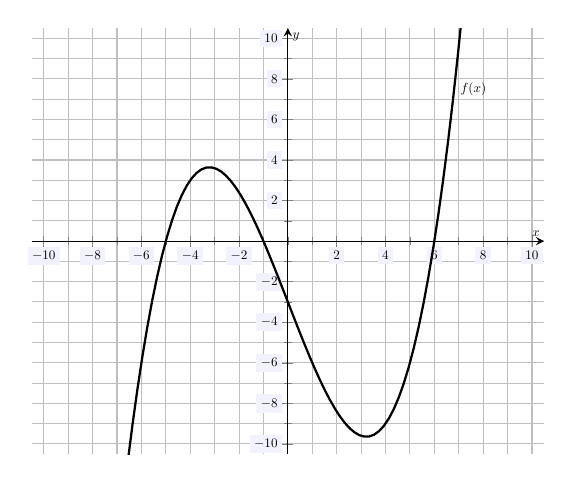
\begin{tikzpicture}[scale=0.95,every node/.style={scale=0.5}]
	\begin{axis}[
	grid=both,
	axis lines=middle,
	ticklabel style={fill=blue!5!white},
	xmin= -10.5, xmax=10.5,
	ymin= -10.5, ymax=10.5,
	xtick={-10,-8,...,10},
	ytick={-10,-8,...,10},
	minor tick = {-10,-9,...,10},
	xlabel=\(x\),ylabel=\(y\),
	]
	\node at (7.6,7.5) {$f(x)$};
	\addplot[line width= 0.03cm,samples=100,domain= -10:10] ({x},{1/10*(x+1)*(x + 5)*(x-6)});

	\end{axis}
	\end{tikzpicture}
	}
\end{minipage}\begin{minipage}[b]{0.48\textwidth}
\wans{The function $f(x)$ does not have an inverse because the graph of $f(x)$ fails the Horizontal Line Test; that is, not every horizontal line intersects the graph of $f(x)$ at most once.} \pvspace{2cm} 
\end{minipage}

\end{document}